\documentclass[conference]{IEEEtran} 

% ---------- Packages ----------
\usepackage{graphicx}
\usepackage{amsmath}
\usepackage{newtxtext,newtxmath} % XeLaTeXでTimes系を安定使用
\usepackage{siunitx}
\usepackage{xcolor}
\usepackage{tikz} % ダミー図用
% 使うTikZライブラリ
\usetikzlibrary{calc,arrows.meta}

% 例:スタイル[leak]を定義(必要に応じて調整)
\tikzset{
  leak/.style = {-{Latex[length=2mm]}, line width=0.4pt}
}
\usepackage[hidelinks]{hyperref}
\usepackage{graphicx}
\graphicspath{{figures/}} % 図のデフォルト検索パス

% === plots ===
\usepackage{pgfplots}
\pgfplotsset{compat=1.18}
\usepackage{pgfplotstable}
\usepackage{tikz} % (pgfplotsが内部で読むが明示しておくと安心)

% ---------- Helper: ダミー図コマンド ----------
\newcommand{\yielddummyfigure}[1][\columnwidth]{%
  \begin{tikzpicture}
    \draw[gray!60,fill=gray!10] (0,0) rectangle (#1,0.6*#1);
    \draw[gray!60] (0.1*#1,0.1*0.6*#1) rectangle (0.9*#1,0.9*0.6*#1);
    \node at (0.5*#1,0.3*#1) {\small DUMMY FIGURE: Yield vs. Lot};
  \end{tikzpicture}%
}

% ---------- Title & Author ----------
\title{Historical Case Study: 0.25-\si{\micro\meter} 64-Mbit DRAM Ramp-up and Pseudo-SRAM (VSRAM)}
\author{
\IEEEauthorblockN{Shinichi Samizo}
\IEEEauthorblockA{Independent Semiconductor Researcher\\
Project Design Hub, Samizo-AITL\\
\textit{Email:} \href{mailto:shin3t72@gmail.com}{shin3t72@gmail.com} \quad
\textit{GitHub:} \href{https://github.com/Samizo-AITL}{Samizo-AITL}}
}

\begin{document}
\maketitle

% ---------- Abstract ----------
\begin{abstract}
This paper presents a flagship proof-of-concept humanoid robot control system that integrates
finite state machines (FSM), proportional-integral-derivative (PID) controllers, state-space methods
(LQR/LQG), and large language models (LLMs) into a unified three-layer architecture. 
Unlike existing humanoid platforms such as Boston Dynamics Atlas and Tesla Optimus,
our approach emphasizes autonomy, fault tolerance, and sustainability.

The proposed architecture is realized as a cross-node chipset design: 
a 22 nm SoC executes LLM inference, FSM management, and state-space control;
a 0.18 µm AMS sensor hub processes multimodal inputs (vision, IMU, force, audio);
and a 0.35 µm LDMOS power drive with external GaN/MOSFET chips delivers high-torque actuation.
Energy harvesting via piezoelectric, photovoltaic, and regenerative methods 
extends operational lifetime in off-grid environments.

System-level modeling and verification are performed using SystemDK, 
demonstrating posture recovery within 200 ms, gait stability improved by 30\% over PID-only control,
and energy efficiency gains of 15\% with hybrid control and harvesting. 
Checkpointing with FRAM/EEPROM further enables fast resume ($\leq$10 ms) and robust mission continuity. 
These results highlight the feasibility of a sustainable and resilient humanoid control system
that bridges advanced control theory with emerging AI techniques.

\end{abstract}


% ---------- Sections ----------
% sections/intro.tex

\section{Introduction}

Memory hierarchies are central to computing systems. 
DRAM remains the dominant volatile memory due to speed, density, and scalability \cite{choi2022,kim2021_dram}. 
However, DRAM scaling faces limits as capacitors shrink; 3D DRAM concepts are explored to extend scaling \cite{iedm2023_dram}.

In parallel, doped HfO$_2$ ferroelectrics enabled FeRAM and FeFET with CMOS-friendly integration \cite{boscke2011,mueller2012}. 
These offer non-volatility with fast switching but face polarization variability, endurance, and TDDB concerns. 

This review contrasts DRAM and FeRAM at device and system levels and outlines hybrid use-cases. 
As an overview, Figs.~\ref{fig:speed_retention} and \ref{fig:energy_speed} conceptually illustrate the trade-offs in access speed, retention, and write energy, which will be detailed in Sec.~\ref{sec:comparison}.

\section{Background}
This work builds on the author's 1997–1998 ramp activities at Epson's Sakata fab under technology transfer from Mitsubishi; details are summarized in the Introduction and referenced archives.

\section{Process Overview and Ramp-up Method}

\subsection{Process Overview (0.25-\si{\micro\meter} 64~Mbit DRAM, 3rd Gen)}

\begin{itemize}
  \item \textbf{Lithography}: First adoption of a KrF stepper for 0.25-\si{\micro\meter} volume exposure.
  \item \textbf{Isolation}: Semi-recess LOCOS.
  \item \textbf{Wells}: Triple-well with Deep N-Well to improve cell noise immunity.
  \item \textbf{Word-Line Gate Electrode}: CVD tungsten silicide (WSi). A dielectric \textbf{barrier cap (BRAC)} sits atop the WL stack, providing etch robustness and insulation.
  \item \textbf{Bit Line}: \emph{Self-aligned contact} --- the bit-line contact and the bit line are formed simultaneously by WSi-CVD; the BRAC blocks contact-to-WL shorts.
  \item \textbf{Storage Node Capacitor}: Stacked capacitor; surface roughening yields $\sim$1.5–1.8$\times$ capacitance gain.
  \item \textbf{Metallization/Passivation}: AlCu/TiN interconnect; SOG planarization; SiN or PI passivation.
\end{itemize}

\subsection{Ramp-up Method}

The node transfer followed a factory-wide, fast-turn scheme:

\paragraph{Base flow: SCF $\rightarrow$ shape lots $\rightarrow$ production lots}
\begin{enumerate}
  \item \textbf{Short Cycle Feedback (SCF)}: Each unit process (diffusion, CVD/PVD, etch, etc.) runs short-cycle wafers per its ramp-up spec to quickly evaluate and lock conditions.
  \item \textbf{Shape lots ($\sim$10 lots)}: Provide \emph{real product wafers} to unit teams for items only assessable on full stacks and, in parallel, (i) verify photo CDs, (ii) photo$\to$etch CD transfer, and (iii) cross-sections after interlayer films. Recipes are updated for following lots.
  \item \textbf{Production (reliability) lots}: Multiple lots for wafer test and long-term reliability (incl.\ burn-in) to judge mass-production readiness.
\end{enumerate}

\paragraph{Practical flow (author's role)}
Process conditions (two floppy disks) were received from the mother fab and deployed to unit teams; each team executed SCF and fed back updates. The author consolidated the latest settings into the \emph{electronic traveler}, launched $\sim$10 shape lots, fixed target CDs/films, and then ran 5 reliability lots for E-test and reliability signoff.

\paragraph{Operations to compress schedule}
Normal lots use stocker $\leftrightarrow$ rail transfer and queue at tools. For critical first-pass lots, we used \textbf{hand-carry flow}: engineers delivered cassettes to tools with operators standing by, eliminating transfer/queue loss. Even so, a full pass took about two months; the entire ramp spanned $\sim$5 months. Daily morning meetings posted a laminated traveler on a whiteboard to visualize lot progress, schedule slip (in days), and unit-team status. Technical staff also operated in a two-shift scheme (day/night) to sustain 24/7 feedback.

\section{Failure Analysis and Yield Improvement}

\subsection{Initial Observation}
The first production lots showed $\sim$65\% yield. Wafer test was dominated by \textbf{Pause Refresh Fail (Bin5)}. Defects appeared as uniformly scattered single-bit errors across the wafer (weak clustering, no edge/line signature). Storage-node capacitance met spec; SEM cross-sections at failed cells revealed no structural anomaly. Other CDs/films/electricals were within spec.

\begin{figure}[t]
  \centering
  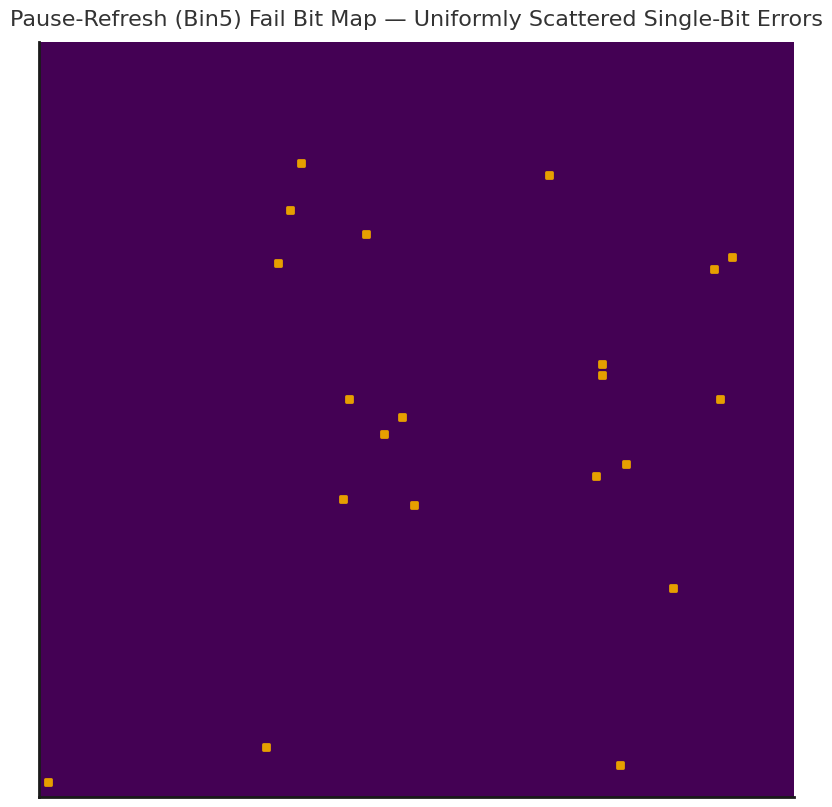
\includegraphics[width=\columnwidth]{fail_bitmap_bin5}
  \caption{Typical fail bit map under pause-refresh test (Bin5).
  Uniformly scattered single-bit errors are observed without edge/line signatures.}
  \label{fig:fail_bitmap}
\end{figure}

\subsection{Hypothesis (Failure Model)}
Directly measurable leakages were normal, suggesting a subtle leakage path. We hypothesized increased leakage at the \textbf{storage-node contact $n^+/p^-$ junction}. After gate etch, a remnant gate oxide on S/D active is repeatedly exposed to resist-stripping \emph{ashing} during multiple LDD steps. Cumulative plasma damage makes the oxide locally porous and can extend damage into the diffusion, creating minute leakage paths. This explains random single-bit distribution without visible structural defects.

% === Storage-node contact n+/p- leakage (TikZ) ===
% === Fig.2 Storage-node contact n+/p- leakage (pure TikZ, minimal IEEE style) ===
\begin{figure}[t]
\centering
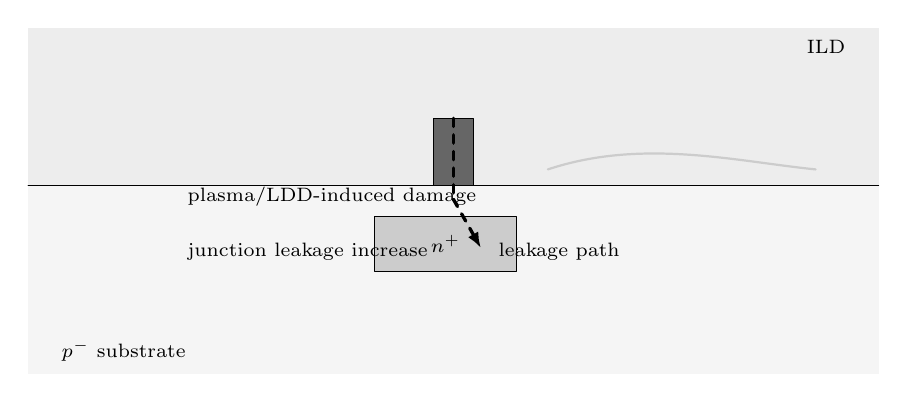
\begin{tikzpicture}[x=1cm,y=1cm,line cap=round,line join=round]
  % 色(グレースケール)
  \def\colILD{black!7}    % ILD淡グレー
  \def\colSub{black!4}    % p-基板の淡グレー
  \def\colDiff{black!20}  % n+拡散
  \def\colLOCOS{black!20} % LOCOS輪郭
  \def\colMetal{black!60} % 金属プラグ

  % キャンバス範囲
  \path (-4.8,-2.4) rectangle (6.0,2.0);

  % ---- ILD(上部帯)----
  \fill[\colILD] (-4.8,0) rectangle (6.0,2.0);
  \node[anchor=east, font=\scriptsize] at (5.7,1.75) {ILD};

  % ---- 基板と表面 ----
  \fill[\colSub] (-4.8,-2.4) rectangle (6.0,0);
  \draw (-4.8,0) -- (6.0,0);
  \node[anchor=west, font=\scriptsize] at (-4.5,-2.1) {$p^{-}$ substrate};

  % ---- LOCOS(右側の鳥のくちばし風プロファイル)----
  \draw[\colLOCOS, line width=0.8pt]
    (1.8,0.20) .. controls (3.0,0.60) and (4.2,0.30) .. (5.2,0.20);

  % ---- n+拡散(ストレージ側)----
  \fill[\colDiff] ( -0.4,-1.1) rectangle (1.4,-0.4);
  \draw ( -0.4,-1.1) rectangle (1.4,-0.4);
  \node[font=\scriptsize] at (0.5,-0.75) {$n^{+}$};

  % ---- ストレージノード・コンタクトプラグ ----
  \fill[\colMetal] (0.35,0.00) rectangle (0.85,0.85);
  \draw (0.35,0.00) rectangle (0.85,0.85);

  % ---- 破線リークパス(コンタクト端→接合)----
  \draw[very thick, dashed] (0.60,0.85) -- (0.60,-0.18);
  \draw[very thick, dashed, -{Latex[length=2mm]}] (0.60,-0.18) -- (0.95,-0.80);
  \node[anchor=west, font=\scriptsize] at (1.05,-0.85) {leakage path};

  % ---- 注記(最小限)----
  \node[anchor=west, font=\scriptsize] at (-2.9,-0.15) {plasma/LDD-induced damage};
  \node[anchor=west, font=\scriptsize] at (-2.9,-0.85) {junction leakage increase};
\end{tikzpicture}
\caption{Schematic of storage-node contact (n$^+$/p$^-$) leakage.
Damage near the contact edge increases junction leakage, degrading retention.}
\label{fig:storage_contact}
\end{figure}

\subsection{Countermeasures}
\begin{itemize}
  \item \textbf{Process}: Replace resist stripping in LDD steps from plasma ashing to \textbf{wet stripping (sulfuric-based)} to eliminate plasma damage. 
  \item \textbf{Integration hygiene}: Confirm downstream photo cleanliness and avoid residue risks with the wet strip.
\end{itemize}

\subsection{Effectiveness}
Yield improved from $\sim$65\% to \textbf{$\sim$80\%}. Uniformly scattered single-bit fails decreased markedly. Burn-in and retention/reliability passed; the final recipe was fixed for volume production.

% === Yield-by-lot (step improvement at countermeasure) ===
\begin{figure}[t]
\centering
\pgfplotstableread[col sep=comma]{data/yield_lot.csv}\yieldtbl
\begin{tikzpicture}
\begin{axis}[
  width=\columnwidth, height=0.58\columnwidth,
  xlabel={Lot ID}, ylabel={Yield [\%]},
  ymin=50, ymax=95,
  xmin=0.5, xmax=12.5,
  grid=both,
  xtick=data,
  xticklabels from table={\yieldtbl}{lot},
  xticklabel style={rotate=45, anchor=east},
]
  % データ描画
  \addplot+[mark=*] table[x expr=\coordindex+1, y=yield]{\yieldtbl};

  % 対策境界: lot04とlot05の間
  \draw[dashed] (axis cs:4.5,50) -- (axis cs:4.5,95);
  \node[anchor=west, font=\footnotesize] at (axis cs:4.55,92)
    {Countermeasure};
\end{axis}
\end{tikzpicture}
\caption{Yield step improvement at the countermeasure boundary
between \texttt{lot04} and \texttt{lot05}. Yield jumps from $\sim$62--63\% 
(lot01--lot04) to $\sim$82--84\% (lot05 onward) after changing 
LDD resist stripping from ashing to wet stripping.}
\label{fig:yield}
\end{figure}
      % ← この中でダミー図を出します
Parallel margin lots efficiently confirmed the process window under mass-line conditions, avoiding delays from strictly serial confirmation. Retention behavior is framed by $\tau = C_{\mathrm{cell}} V_{\mathrm{cell}} / I_{\mathrm{leak}}$, highlighting sensitivity to junction and dielectric leakage. The disturb-refresh behavior connects conceptually to modern row-disturb/row-hammer phenomena. We discuss portability of this ramp-up template to technology transfers beyond DRAM.

% sections/conclusion.tex

DRAM will continue to dominate volatile working memory due to speed, density, and ecosystem maturity. HfO2-based FeRAM/FeFET offers a CMOS-compatible non-volatile complement with fast access, though variability, endurance dispersion, and integration limits remain active topics \cite{noheda2023,martin2020}. Hybrid hierarchies that pair DRAM for hot data with FeRAM for persistence can reduce refresh energy while enabling fast recovery paths.

Looking ahead, co-design across devices, controllers, and operating systems will be central: retention-aware placement, telemetry-driven reliability management, and low-latency persistence paths are promising directions to broaden deployment from embedded and edge to selected data-centric systems.


% ---------- References ----------
\nocite{*} % ひとまずrefs.bibの全項目を出力(不要なら削除)
\bibliographystyle{IEEEtran}
\bibliography{refs}

% ---------- Author Biography ----------
\section*{Author Biography}
\noindent\textbf{Shinichi Samizo}
received the M.S. degree in Electrical and Electronic Engineering from Shinshu University, Japan.
He worked at Seiko Epson Corporation as an engineer in semiconductor memory and mixed-signal device development, and also contributed to inkjet MEMS actuators and PrecisionCore printhead technology.
He is currently an independent semiconductor researcher focusing on process/device education, memory architecture, and AI system integration.
\textbf{Contact:} \href{mailto:shin3t72@gmail.com}{shin3t72@gmail.com}, Samizo-AITL.

\end{document}
